% Z[sqrt 11] drawn via a+b·sqrt11 |-> (a+b·sqrt11, a-b·sqrt11); the red
% hyperbolas |xy|=1 bound the region of norm < 1.
% Source: book/tex/H113/ring-flavors.tex (§ Euclidean domains).
\documentclass[border=2mm]{standalone}
\usepackage{tikz}
\begin{document}
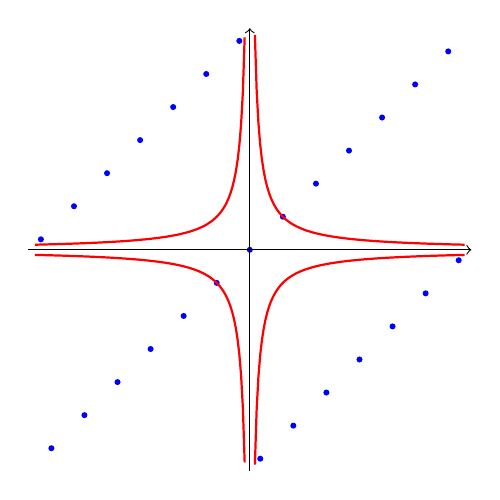
\begin{tikzpicture}[scale=0.42]
  \foreach \a in {-8,...,8}{
    \foreach \b in {-2,...,2}{
      \pgfmathsetmacro{\px}{\a+\b*sqrt(11)}
      \pgfmathsetmacro{\py}{\a-\b*sqrt(11)}
      \pgfmathtruncatemacro{\ok}{(\px>-6.5 && \px<6.5 && \py>-6.5 && \py<6.5)?1:0}
      \ifnum\ok=1 \fill[blue] (\px,\py) circle (2.6pt); \fi
    }
  }
  \draw[red, thick, domain=0.1539:6.5, samples=120] plot (\x,{1/\x});
  \draw[red, thick, domain=-6.5:-0.1539, samples=120] plot (\x,{1/\x});
  \draw[red, thick, domain=0.1539:6.5, samples=120] plot (\x,{-1/\x});
  \draw[red, thick, domain=-6.5:-0.1539, samples=120] plot (\x,{-1/\x});
  \draw[->] (-6.7,0) -- (6.7,0);
  \draw[->] (0,-6.7) -- (0,6.7);
\end{tikzpicture}
\end{document}
